\documentclass[12pt,english,brazil,a4paper,utf8,oneside]{utfpr-tcc}

% carrega o arquivo configuracoes.tex que contém os pacotes e comandos Latex.
%
% Esse arquivo conterá pacotes e comandos utilizados na monografia
%
% Observação - devido a um erro do sharelatex foi necessário colocar na raiz do projeto os seguintes arquivos:
% gcnumparser.sty, fcprefix.sty, fmtcount.sty, fc-poruges.def, fcportuguese.def.
% Tal problema foi relatado em: https://github.com/nlct/fmtcount/issues/26
% Quando o sharelatex corrigir o problema acredito que podemos remover esses arquivos do projeto. At. Luiz Arthur.
%

% Este comando não é necessário: utilizei apenas para deixar o latex2rtf
% feliz (e descobrir a codificação do texto).
\usepackage[utf8]{inputenc}

% Suporte a figuras e subfiguras
\usepackage{graphics}
\usepackage{subfigure}

% Suporte a tabelas (principalmente do cronograma)
\usepackage{tabularx}
\usepackage{multirow}
\usepackage{array}
\usepackage{tabularx}
\usepackage{colortbl}
\usepackage{hhline}
\usepackage{xcolor}

% Escalar fontes para redimencionar, por exemplo tabelas
\usepackage{scalefnt}

% Algoritmos.
\usepackage{algorithm,algorithmic}

\usepackage[alf]{abntex2cite}

% Elementos geralmente utilizados na tabela do cronograma
\newcommand{\fullcell}{\multicolumn{1}{>{\columncolor[gray]{0.5}}c}{}}
\newcommand{\fullcellline}{\multicolumn{1}{>{\columncolor[gray]{0.5}}c|}{}}
\newcommand{\mc}[3]{\multicolumn{#1}{#2}{#3}}
\newcommand{\y}{\rule{8pt}{4pt}}
\newcommand{\n}{\hspace*{8pt}}

% Define o caminho das figuras
\graphicspath{{images/}}

%% Configuração de glossário
\usepackage[portuguese]{nomencl}
\usepackage[nogroupskip,acronym,nomain,nonumberlist,nopostdot,nohypertypes={acronym}]{glossaries}

\makenoidxglossaries

% para siglas em português
\newcommand{\sigla}[2]
{
 \newglossaryentry{#1}{
  name=#1,
  description={#2},
  first={#2 (#1)},
  long={#2}
 }  
}

% para siglas de língua estrangeira, nessas a descrição longa fica em itálico.
\newcommand{\siglaIt}[2]
{
 \newglossaryentry{#1}{
  name=#1,
  description={\textit{#2}},
  first={\textit{#2} ({#1})},
  long={\textit{#2}}
 }  
}

% --- Estilos para apresentação de Código ----- %
\usepackage{listings}
\lstloadaspects{formats}

% Opções de listing usados para o código fonte
% Ref: http://en.wikibooks.org/wiki/LaTeX/Packages/Listings

\lstset{ %
language=Java,                  % choose the language of the code
basicstyle=\footnotesize,       % the size of the fonts that are used for the code
%basicstyle=\ttfamily,
stringstyle=\ttfamily\color[rgb]{0.16,0.16,0.16},
numbers=left,                   % where to put the line-numbers
numberstyle=\footnotesize,      % the size of the fonts that are used for the line-numbers
stepnumber=1,                   % the step between two line-numbers. If it's 1 each line will be numbered
numbersep=4pt,                  % how far the line-numbers are from the code
showspaces=false,               % show spaces adding particular underscores
showstringspaces=false,         % underline spaces within strings
showtabs=false,                 % show tabs within strings adding particular underscores
frame=single,	                % adds a frame around the code
framerule=0.6pt,
tabsize=2,	                % sets default tabsize to 2 spaces
captionpos=b,                   % sets the caption-position to bottom
breaklines=true,                % sets automatic line breaking
breakatwhitespace=false,        % sets if automatic breaks should only happen at whitespace
escapeinside={\%*}{*)},         % if you want to add a comment within your code
backgroundcolor=\color[rgb]{1.0,1.0,1.0}, % choose the background color.
rulecolor=\color[rgb]{0.8,0.8,0.8},
extendedchars=true,
xleftmargin=10pt,
xrightmargin=10pt,
framexleftmargin=10pt,
framexrightmargin=10pt
}

\definecolor{javared}{rgb}{0.6,0,0} % for strings
\definecolor{javagreen}{rgb}{0.25,0.5,0.35} % comments
\definecolor{javapurple}{rgb}{0.5,0,0.35} % keywords
\definecolor{javadocblue}{rgb}{0.25,0.35,0.75} % javadoc

\definecolor{DarkBlue}{rgb}{0,0,0.61}
\definecolor{DarkGreen}{rgb}{0,0.4,0}

% Numeros.
\lstdefinestyle{mynumbers}{
	numbers=left,
	stepnumber=1,
	numbersep=4pt,
	numberstyle=\tiny\color{black}
}
% Text Code.
\lstdefinestyle{mytextcode}{
	basicstyle=\footnotesize,
	tabsize=2,
	showspaces=false,
	showstringspaces=false,
	extendedchars=true,
	breaklines=true
}
% Frame.
\lstdefinestyle{myframe}{
	backgroundcolor=\color{white},
	frame=trbl
}
% C++ Style.
\lstdefinestyle{C++}{
	language=C++,
	style=mynumbers,
	style=mytextcode,
	style=myframe,
  keywordstyle=\color{black}\bfseries,
  stringstyle=\color{gray},
  commentstyle=\color[rgb]{0.08,0.08,0.08},
  morecomment=[s][\color{lightgray}]{/*}{*/},
  otherkeywords={\#include, \#define, \#pragma, \#typedef, dim3},
  emph={ __device__, __global__, __shared__, __host__, __constant__},
  emphstyle=\color{DarkBlue}\bfseries,
  emph={[2] printf, scanf},
  emphstyle=[2]\color{DarkGreen},
}
% C Style.
\lstdefinestyle{C}{
	language=C,
	style=mynumbers,
	style=mytextcode,
	style=myframe,
	keywordstyle=\color{black}\bfseries,
  	stringstyle=\color{gray},
  	commentstyle=\color[rgb]{0.08,0.08,0.08},
  	morecomment=[s][\color{lightgray}]{/*}{*/},
  	otherkeywords={\#include, \#define, \#pragma, \#typedef, dim3, bool},
  	emph={ __device__, __global__, __shared__, __host__, __constant__},
  	emphstyle=\color{DarkBlue}\bfseries,
  	emph={[2] printf, scanf},
  	emphstyle=[2]\color{DarkGreen},
	backgroundcolor={}
}
% Bash Style.
\lstdefinestyle{bash}{
	language=bash,
	style=mynumbers,
	style=mytextcode,
	style=myframe,
	backgroundcolor={},
	frame=single,
	basicstyle=\scriptsize\ttfamily
}
% Python Style.
\lstdefinestyle{python}{
	language=python,
	style=mynumbers,
	style=mytextcode,
	style=myframe,
	backgroundcolor={}
}
% Java Style.
\lstdefinestyle{java}{
	language=java,
	style=mynumbers,
	style=mytextcode,
	style=myframe,
	backgroundcolor={}
}
% ASM Style.
\lstdefinestyle{asm}{
  %belowcaptionskip=1\baselineskip,
  %xleftmargin=\parindent,
  language=[x86masm]Assembler,
  style=mynumbers,
  style=mytextcode,
  style=myframe,
  backgroundcolor={},
  frame=single,
  basicstyle=\scriptsize\ttfamily,
  commentstyle=\itshape\color{purple!40!black},
}

% Fortran Style.
\lstdefinestyle{fortran}{
  language=[90]Fortran,
  style=mynumbers,
  style=mytextcode,
  style=myframe,
  backgroundcolor={},
  frame=single,
  basicstyle=\footnotesize,
  commentstyle=\itshape\color{purple!40!black},
  morecomment=[l]{!\ }% Comment only with space after !
}

% LLVM Style.
\lstdefinestyle{llvm}{
	language=llvm,
	%inputencoding=utf8,
	style=mynumbers,
	style=mytextcode,
	style=myframe,
	backgroundcolor={},
	frame=single,
	basicstyle=\scriptsize\ttfamily,
  tabsize=4,
  %rulecolor=,
  upquote=true,
% aboveskip={1.5\baselineskip},
  columns=fixed,
  prebreak = \raisebox{0ex}[0ex][0ex]{\ensuremath{\hookleftarrow}},
  showtabs=false,
	%basicstyle=\scriptsize\upshape\ttfamily,
  identifierstyle=\ttfamily,
  keywordstyle=\ttfamily\bfseries\color[rgb]{0,0,0},
  %commentstyle=\ttfamily\color[rgb]{0.133,0.545,0.133},
  commentstyle=\ttfamily\color[rgb]{0.08,0.08,0.08},
  %stringstyle=\ttfamily\color[rgb]{0.627,0.126,0.941}
  stringstyle=\ttfamily\color[rgb]{0.16,0.16,0.16}
}

\lstdefineformat{C}{%
	\{=\newline\string\newline\indent,%
	\}=[;]\newline\noindent\string\newline,%
	\};=\newline\noindent\string\newline,%
	;=[\ ]\string\space}

% --- Fim da Definição de Estilos para apresentação de Código ----- %
% carrega o arquivo constantes.tex que contém dados do curso/monografia que NÃO DEVEM ser alterados. 
% Dados do curso que não precisam de alteração
\university{Universidade Tecnológica Federal do Paraná}
\universityen{Federal University of Technology -- Paraná}
\universityunit{Departamento Acadêmico de Computação}
\address{Campo Mourão}
\addressen{Campo Mourão, PR, Brazil}
\documenttype{Monografia}
\documenttypeen{Monograph}
\degreetype{Graduação}
% carrega o arquivo variaveis.tex que contém dados do acadêmico/monografia que DEVEM ser alterados.
% Dados do curso. Caso seja BCC:
\program{Curso de Bacharelado em Ciência da Computação}
\programen{Undergradute Program in Computer Science}
\degree{Bacharel}
\degreearea{Ciência da Computação}
% Caso seja TSI:
% \program{Curso Superior de Tecnologia em Sistemas para Internet}
% \programen{Undergradute Program in Tecnology for Internet Systems}
% \degree{Tecnólogo}
% \degreearea{Tecnologia em Sistemas para Internet}


% Dados da disciplina. Escolha uma das opções e a descomente:
% TCC1:
\goal{Proposta de Trabalho de Conclusão de Curso de Graduação}
\course{Trabalho de Conclusão de Curso 1}
% TCC2:
% \goal{Trabalho de Conclusão de Curso de graduação}
% \course{Trabalho de Conclusão de Curso 2}


% Dados do TCC (precisa alterar)
\author{Otávio Silva Goes}  % Seu nome
\title{Sistema de Recomendação para Ameaças de Cibersegurança} % Título do trabalho
\titleen{Cybersecurity Threats Recommender System} % Título traduzido para inglês
\advisor{Prof. Dr. Rodrigo Campiolo} % Nome do orientador. Lembre-se de prefixar com "Prof. Dr.", "Profª. Drª.", "Prof. Me." ou "Profª. Me."}
% \coadvisor{} % Nome do coorientador, caso exista. Caso não exista, comente a linha.
\depositshortdate{2017} % Ano em que depositou este documento

% Dados da ficha catalografica. Ela é opcional, mas é uma boa ideia inserí-la. Exemplos para geração (http://fichacatalografica.sibi.ufrj.br/)
\fichacatautor{GOES, Otávio}  % Nome conforme citado (ou seja, no formato "Sobrenome, Nome").
\fichacatbib{Biblioteca da UTFPR de Campo Mourão} % Não alterar
\fichacatpum{M488} % Código Cutter-Sanborn. Use a primeira letra do sobrenome seguido do número conforme as primeiras letras do sobrenome e a tabela http://www.amormino.com.br/cutter-sanborn/cutter1.html
\fichacatpalcha{} % Assuntos do trabalho. Cada item deve ser enumerado e separado por ponto: 1. xxx. 2. yyy. 3. zzz.
\fichacatpdois{} % Deixar em branco

% carrega o arquivo listaabreviaturas.tex que está dentro do diretório pretextual, esse arquivo contém as siglas utilizadas na monografia.
% quando a sigla for de língua portuguesa utilize \sigla{SIGLA}{Significado em português}
% quando a sigla for de língua estrangeira utilize \siglaIt{SIGLA}{Significado em Inglês}

\sigla{UTFPR}{Universidade Tecnológica Federal do Paraná}
\siglaIt{ACM}{Association for Computing Machinery}
\siglaIt{IP}{Internet Protocol}
\siglaIt{TCP}{Transmission Control Protocol}


% No texto quando for utilizar a sigla utilize os seguintes comandos:
%\acrlong{label} - acronimo/sigla longo
%\acrshort{label} - acronimo/sigla curta
%\Gls{TCP} - sigla com o significado primeiro em Maiusculo
%\GLS{TCP} - sigla com o significado tudo em MAIUSCULO
%\gls{TCP} - sigla com o significado tudo em minusculo % usando glossaries

\begin{document}
	
\frontmatter
\maketitle

% Dedicatória é opcional, para usar descomentar a linha a seguir e edite o arquivo pretextual/dedicatoria.tex
\dedicate{Para minha mãe, para meu pai e para você...} % Opcional - descomentar para usar

% Agradecimento é opcional, para usar descomentar a linha a seguir e edite o arquivo pretextual/dedicatoria.tex
\begin{agradecimentos}

agradeço agradeço agradeço agradeço agradeço agradeço agradeço agradeço  agradeço agradeço agradeço agradeço agradeço agradeço agradeço agradeço agradeço agradeço agradeço agradeço agradeço agradeço agradeço agradeço agradeço agradeço agradeço agradeço agradeço agradeço agradeço agradeço agradeço agradeço agradeço agradeço agradeço agradeço agradeço agradeço agradeço agradeço agradeço agradeço agradeço agradeço agradeço agradeço agradeço agradeço agradeço agradeço agradeço agradeço agradeço agradeço agradeço agradeço agradeço agradeço agradeço agradeço agradeço agradeço agradeço agradeço agradeço agradeço agradeço agradeço agradeço agradeço 

\end{agradecimentos} % Opcional - descomentar para usar

% carrega o arquivo resumo.tex que está dentro do diretório pretextual, esse arquivo deve conter o resumo da monografia.
\begin{resumo}
%Elemento obrigatório, constituído de uma sequência de frases concisas e objetivas, em forma de texto.  Deve apresentar os objetivos, métodos empregados, resultados e conclusões.  O resumo deve ser redigido em parágrafo único, conter no máximo 500 palavras e ser seguido dos termos representativos do conteúdo do trabalho (palavras-chave).


TEXTO TEXTO TEXTO TEXTO TEXTO TEXTO TEXTO TEXTO TEXTO TEXTO TEXTO TEXTO TEXTO TEXTO TEXTO TEXTO TEXTO TEXTO TEXTO TEXTO TEXTO TEXTO TEXTO TEXTO TEXTO TEXTO TEXTO TEXTO TEXTO TEXTO TEXTO TEXTO TEXTO TEXTO TEXTO TEXTO TEXTO TEXTO TEXTO TEXTO TEXTO TEXTO TEXTO TEXTO TEXTO TEXTO TEXTO TEXTO TEXTO TEXTO TEXTO TEXTO TEXTO TEXTO TEXTO TEXTO TEXTO TEXTO TEXTO TEXTO TEXTO TEXTO TEXTO TEXTO TEXTO TEXTO TEXTO TEXTO TEXTO TEXTO TEXTO TEXTO TEXTO TEXTO TEXTO TEXTO TEXTO TEXTO TEXTO TEXTO TEXTO TEXTO TEXTO TEXTO TEXTO TEXTO TEXTO TEXTO TEXTO TEXTO TEXTO TEXTO TEXTO TEXTO TEXTO TEXTO TEXTO TEXTO TEXTO TEXTO TEXTO TEXTO TEXTO TEXTO TEXTO TEXTO TEXTO TEXTO TEXTO TEXTO TEXTO TEXTO TEXTO TEXTO TEXTO TEXTO TEXTO TEXTO TEXTO TEXTO TEXTO TEXTO TEXTO TEXTO TEXTO TEXTO TEXTO TEXTO TEXTO TEXTO TEXTO TEXTO

% TODO: se possível, escreva um resumo estruturado. Para TCC 1, o resumo estruturado teria os seguintes elementos:
% \textbf{Contexto:} \\
% \textbf{Objetivo:} \\
% \textbf{Método:} \\
% \textbf{Resultados esperados:} 
% ou, para TCC 2:
% \textbf{Contexto:} \\
% \textbf{Objetivo:} \\
% \textbf{Método:} \\
% \textbf{Resultados:} \\
% \textbf{Conclusões:}

% Palavras-chaves, separadas por ponto (tente não definir mais do que cinco)
\palavraschaves{}
\end{resumo}
% carrega o arquivo abstract.tex que está dentro do diretório pretextual, esse arquivo deve conter um resumo escrito na linguá inglesa para a monografia.
% Caso seja TCC 2, precisa traduzir o resumo e as palavras-chaves para inglês:
\begin{abstract}
Put the abstract here...

TEXT TEXT TEXT TEXT TEXT TEXT TEXT TEXT TEXT TEXT TEXT TEXT TEXT TEXT TEXT TEXTTEXT TEXT TEXT TEXT TEXT TEXT TEXT TEXTTEXT TEXT TEXT TEXT TEXT TEXT TEXT TEXTTEXT TEXT TEXT TEXT TEXT TEXT TEXT TEXTTEXT TEXT TEXT TEXT TEXT TEXT TEXT TEXTTEXT TEXT TEXT TEXT TEXT TEXT TEXT TEXTTEXT TEXT TEXT TEXT TEXT TEXT TEXT TEXTTEXT TEXT TEXT TEXT TEXT TEXT TEXT TEXTTEXT TEXT TEXT TEXT TEXT TEXT TEXT TEXTTEXT TEXT TEXT TEXT TEXT TEXT TEXT TEXTTEXT TEXT TEXT TEXT TEXT TEXT TEXT TEXTTEXT TEXT TEXT TEXT TEXT TEXT TEXT TEXTTEXT TEXT TEXT TEXT TEXT TEXT TEXT TEXTTEXT TEXT TEXT TEXT TEXT TEXT TEXT TEXTTEXT TEXT TEXT TEXT TEXT TEXT TEXT TEXT
% \textbf{Context:}
% \textbf{Objective:}
% \textbf{Method:}
% \textbf{Results:}
% \textbf{Conclusions:}

% Palavras-chaves em inglês, separadas por ponto.
% \keywords{}
\end{abstract}

% Listas (opcionais, mas recomenda-se a partir de 5 elementos)
\listoffigures
\listoftables
%\listofacronyms
\printnoidxglossaries

% Sumário
\tableofcontents

\mainmatter

% Capítulos da monografia:
\chapter{Introdução}
\label{cap:introducao}

Coloque aqui o texto da introdução, contextualizando o seu trabalho...

Testando o uso das siglas na - pela primeira vez para \gls{ACM}. Segunda vez para \gls{ACM}...

blabla... \gls{UTFPR}

xxx \gls{TCP}

\acrlong{UTFPR}

A rede \gls{IP}...

% Sugestões de seções
\section{Considerações preliminares}

Aqui você pode descrever problemas, soluções e outros assuntos que ajudem a introduzir o leitor ao contexto de seu trabalho...

(ATENÇÃO - Essa seção é uma sugestão, veja com o seu orientador se você vai ter essa e se vai ter esse nome!)

TEXTO TEXTO TEXTO TEXTO TEXTO TEXTO TEXTO TEXTO TEXTO TEXTO TEXTO TEXTO TEXTO TEXTO TEXTO TEXTO TEXTO TEXTO TEXTO TEXTO TEXTO TEXTO TEXTO TEXTO TEXTO TEXTO TEXTO TEXTO TEXTO TEXTO TEXTO TEXTO TEXTO TEXTO TEXTO TEXTO TEXTO TEXTO TEXTO TEXTO TEXTO TEXTO TEXTO TEXTO TEXTO TEXTO TEXTO TEXTO TEXTO TEXTO TEXTO TEXTO TEXTO TEXTO TEXTO TEXTO TEXTO TEXTO TEXTO TEXTO TEXTO TEXTO TEXTO TEXTO TEXTO TEXTO TEXTO TEXTO TEXTO TEXTO TEXTO TEXTO TEXTO TEXTO TEXTO TEXTO TEXTO TEXTO TEXTO TEXTO TEXTO TEXTO TEXTO TEXTO TEXTO TEXTO TEXTO TEXTO TEXTO TEXTO TEXTO TEXTO TEXTO TEXTO TEXTO TEXTO TEXTO TEXTO TEXTO TEXTO TEXTO TEXTO TEXTO TEXTO TEXTO TEXTO TEXTO TEXTO TEXTO TEXTO TEXTO TEXTO TEXTO TEXTO TEXTO TEXTO TEXTO TEXTO TEXTO TEXTO TEXTO TEXTO TEXTO TEXTO TEXTO TEXTO TEXTO TEXTO TEXTO TEXTO TEXTO TEXTO

\section{Problema de Pesquisa}
\label{cap:introducao:sec:problema:pesquisa}

Descreva o seu Problema de Pesquisa com as questões de pesquisa que seu trabalho irá tentar responder.

\section{Objetivos}
\label{cap:introducao:sec:objetivos}

Descreva de maneira sucinta os objetivos de seu trabalho (o que você fará durante o desenvolvimento de TCC 1 e TCC 2?). Faça um texto BEM curto e objetivo...

(ATENÇÃO - Essa seção é uma sugestão, veja com o seu orientador se você vai ter essa e se vai ter esse nome!)

TEXTO TEXTO TEXTO TEXTO TEXTO TEXTO TEXTO TEXTO TEXTO TEXTO TEXTO TEXTO TEXTO TEXTO TEXTO TEXTO TEXTO TEXTO TEXTO TEXTO TEXTO TEXTO TEXTO TEXTO TEXTO TEXTO TEXTO TEXTO TEXTO TEXTO TEXTO TEXTO TEXTO TEXTO TEXTO TEXTO TEXTO TEXTO TEXTO TEXTO TEXTO TEXTO TEXTO TEXTO TEXTO TEXTO TEXTO TEXTO TEXTO TEXTO TEXTO TEXTO TEXTO TEXTO TEXTO TEXTO TEXTO TEXTO TEXTO TEXTO TEXTO TEXTO TEXTO TEXTO TEXTO TEXTO TEXTO TEXTO TEXTO TEXTO TEXTO TEXTO TEXTO TEXTO TEXTO TEXTO TEXTO TEXTO TEXTO TEXTO TEXTO TEXTO TEXTO TEXTO TEXTO TEXTO TEXTO TEXTO TEXTO TEXTO TEXTO TEXTO TEXTO TEXTO TEXTO TEXTO TEXTO TEXTO TEXTO TEXTO TEXTO TEXTO TEXTO TEXTO TEXTO TEXTO TEXTO TEXTO TEXTO TEXTO TEXTO TEXTO TEXTO TEXTO TEXTO TEXTO TEXTO TEXTO TEXTO TEXTO TEXTO TEXTO TEXTO TEXTO TEXTO TEXTO TEXTO TEXTO TEXTO TEXTO TEXTO TEXTO

\section{Contribuições}
\label{cap:introducao:sec:contribuicoes}

No que o seu trabalho ajuda? Há diferenças entre o seu trabalho e outros?

(ATENÇÃO - Essa seção é uma sugestão, veja com o seu orientador se você vai ter essa e se vai ter esse nome!)

TEXTO TEXTO TEXTO TEXTO TEXTO TEXTO TEXTO TEXTO TEXTO TEXTO TEXTO TEXTO TEXTO TEXTO TEXTO TEXTO TEXTO TEXTO TEXTO TEXTO TEXTO TEXTO TEXTO TEXTO TEXTO TEXTO TEXTO TEXTO TEXTO TEXTO TEXTO TEXTO TEXTO TEXTO TEXTO TEXTO TEXTO TEXTO TEXTO TEXTO TEXTO TEXTO TEXTO TEXTO TEXTO TEXTO TEXTO TEXTO TEXTO TEXTO TEXTO TEXTO TEXTO TEXTO TEXTO TEXTO TEXTO TEXTO TEXTO TEXTO TEXTO TEXTO TEXTO TEXTO TEXTO TEXTO TEXTO TEXTO TEXTO TEXTO TEXTO TEXTO TEXTO TEXTO TEXTO TEXTO TEXTO TEXTO TEXTO TEXTO TEXTO TEXTO TEXTO TEXTO TEXTO TEXTO TEXTO TEXTO TEXTO TEXTO TEXTO TEXTO TEXTO TEXTO TEXTO TEXTO TEXTO TEXTO TEXTO TEXTO TEXTO TEXTO TEXTO TEXTO TEXTO TEXTO TEXTO TEXTO TEXTO TEXTO TEXTO TEXTO TEXTO TEXTO TEXTO TEXTO TEXTO TEXTO TEXTO TEXTO TEXTO TEXTO TEXTO TEXTO TEXTO TEXTO TEXTO TEXTO TEXTO TEXTO TEXTO TEXTO

\section{Organização do Texto}
\label{cap:introducao:sec:organizacao:texto}

No Capítulo~\ref{cap:introducao} blablabla, no capítulo seguinte tititi, etc... Nossa proposta é apresentada no Capítulo~\ref{cap:proposta}.... Finalmente, no Capítulo~\ref{cap:conclusoes} apresentamos as conclusões obtidas no desenvolvimento deste trabalho...

(ATENÇÃO - Essa seção é uma sugestão, veja com o seu orientador se você vai ter essa e se vai ter esse nome!)

TEXTO TEXTO TEXTO TEXTO TEXTO TEXTO TEXTO TEXTO TEXTO TEXTO TEXTO TEXTO TEXTO TEXTO TEXTO TEXTO TEXTO TEXTO TEXTO TEXTO TEXTO TEXTO TEXTO TEXTO TEXTO TEXTO TEXTO TEXTO TEXTO TEXTO TEXTO TEXTO TEXTO TEXTO TEXTO TEXTO TEXTO TEXTO TEXTO TEXTO TEXTO TEXTO TEXTO TEXTO TEXTO TEXTO TEXTO TEXTO TEXTO TEXTO TEXTO TEXTO TEXTO TEXTO TEXTO TEXTO TEXTO TEXTO TEXTO TEXTO TEXTO TEXTO TEXTO TEXTO TEXTO TEXTO TEXTO TEXTO TEXTO TEXTO TEXTO TEXTO TEXTO TEXTO TEXTO TEXTO TEXTO TEXTO TEXTO TEXTO TEXTO TEXTO TEXTO TEXTO TEXTO TEXTO TEXTO TEXTO TEXTO TEXTO TEXTO TEXTO TEXTO TEXTO TEXTO TEXTO TEXTO TEXTO TEXTO TEXTO TEXTO TEXTO TEXTO TEXTO TEXTO TEXTO TEXTO TEXTO TEXTO TEXTO TEXTO TEXTO TEXTO TEXTO TEXTO TEXTO TEXTO TEXTO TEXTO TEXTO TEXTO TEXTO TEXTO TEXTO TEXTO TEXTO TEXTO TEXTO TEXTO TEXTO TEXTO TEXTO
\chapter{Conceitos}
\label{cap:conceitos}

Descreva os conceitos necessários para que o leitor entenda o seu trabalho (referencial teórico). 

Exemplo, se o seu trabalho é a respeito de banco de dados e redes você pode descrever conceitos a respeito desses assuntos ou de assuntos que ajudem ao leitor a entender a sua proposta/metodologia.

(ATENÇÃO - veja com o seu orientador se você vai ter este capítulo e se este vai ter nome!)

TEXTO TEXTO TEXTO TEXTO TEXTO TEXTO TEXTO TEXTO TEXTO TEXTO TEXTO TEXTO TEXTO TEXTO TEXTO TEXTO TEXTO TEXTO TEXTO TEXTO TEXTO TEXTO TEXTO TEXTO TEXTO TEXTO TEXTO TEXTO TEXTO TEXTO TEXTO TEXTO TEXTO TEXTO TEXTO TEXTO TEXTO TEXTO TEXTO TEXTO TEXTO TEXTO TEXTO TEXTO TEXTO TEXTO TEXTO TEXTO TEXTO TEXTO TEXTO TEXTO TEXTO TEXTO TEXTO TEXTO TEXTO TEXTO TEXTO TEXTO TEXTO TEXTO TEXTO TEXTO TEXTO TEXTO TEXTO TEXTO TEXTO TEXTO TEXTO TEXTO TEXTO TEXTO TEXTO TEXTO TEXTO TEXTO TEXTO TEXTO TEXTO TEXTO TEXTO TEXTO TEXTO TEXTO TEXTO TEXTO TEXTO TEXTO TEXTO TEXTO TEXTO TEXTO TEXTO TEXTO TEXTO TEXTO TEXTO TEXTO TEXTO TEXTO TEXTO TEXTO TEXTO TEXTO TEXTO TEXTO TEXTO TEXTO TEXTO TEXTO TEXTO TEXTO TEXTO TEXTO TEXTO TEXTO TEXTO TEXTO TEXTO TEXTO TEXTO TEXTO TEXTO TEXTO TEXTO TEXTO TEXTO TEXTO TEXTO TEXTO

%---------------------------------------------------%
\section{Usando de Figuras}
\label{cap:conceitos:sec:usando:figuras}

Normalmente Figuras e outros objetos são utilizadas no texto para exemplificar ou ilustrar uma ideia ou conceito. Assim não esqueça de referencia-la em seu texto. Não deixe objetos sem serem referenciados no texto em sua monografia. A Figura~\ref{fig:levantamento:requisitos} apresenta ...

\begin{figure}[!htb]
    \centering
    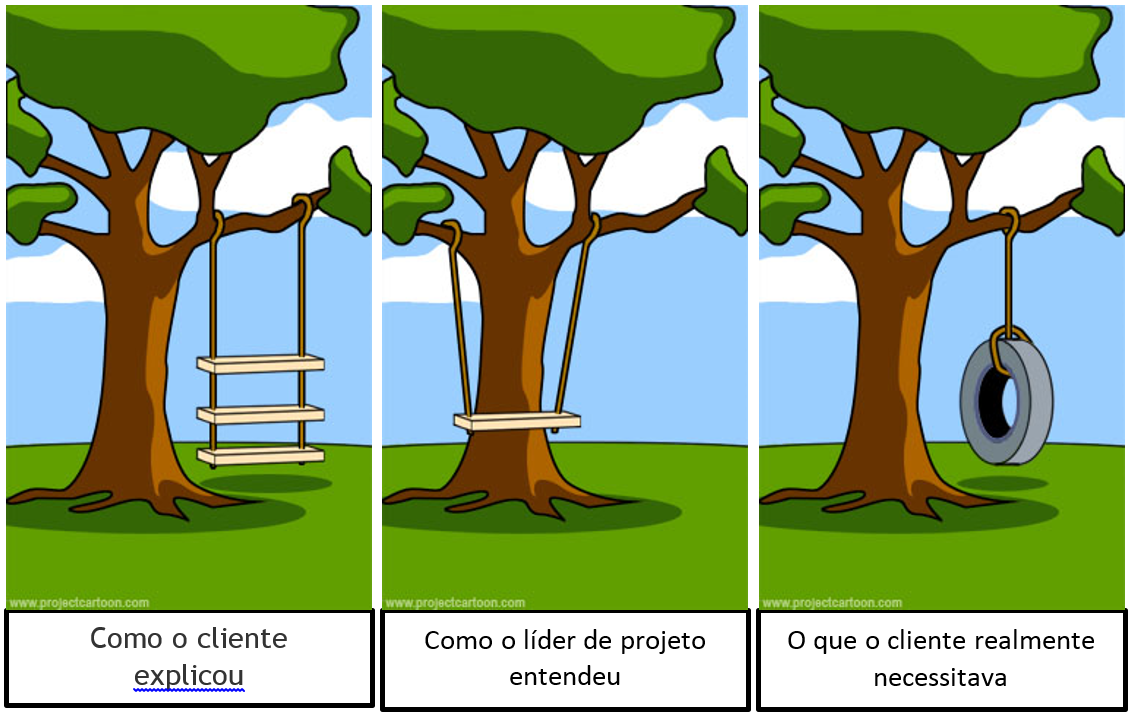
\includegraphics[width=0.90\textwidth]{figuras/The-Project-Cartoon-Beta.png}
    \caption{A importância do Levantamento de Requisitos}
    \label{fig:levantamento:requisitos}
\end{figure}

%---------------------------------------------------%
\section{Exemplo de uso de Equação}
\label{cap:conceitos:sec:usando:equacoes}

O valor mensurado do tráfego de bytes considerando todos os níveis da hierarquia de memória ($Q_{total}$) é calculado usando a Equação \ref{equ:roofline:qtotal}.

\begin{equation}\label{equ:roofline:qtotal}
Q_{total} = Q_{L1} + Q_{L2} + Q_{LLC} + Q_{MEM}
\end{equation}

%---------------------------------------------------%
\section{Usando Código}
\label{cap:conceitos:sec:usando:codigo}

Se for necessário apresentar a ideia de um Algoritmo~\ref{alg:decisao-001} em pseudocódigo...

\begin{algorithm}[H]
	\caption{Meu algoritmo}
	\label{alg:decisao-001}
	\begin{algorithmic}[1]
		\STATE $\textbf{INPUT:}*better\_device\_index$
		\STATE $\textbf{OUTPUT:} *better\_device\_index, offload\_decison$
		\STATE $offload\_decision \leftarrow true$
		\IF{($offload\_decision \leftarrow \textbf{RM\_check\_all\_eventsets\_was\_collected(})$)}
		\STATE $oi \leftarrow \textbf{RM\_get\_operational\_intensity}()$
		\STATE $better\_device\_index \leftarrow \textbf{RM\_get\_better\_device\_to\_execution}(oi)$ 
		\ELSE
		\STATE {$better\_device\_index \leftarrow 0$}	
		\ENDIF
		\RETURN $offload\_decision$
	\end{algorithmic}
\end{algorithm}

O Código~\ref{cod:omp:directive:parallel} apresenta um código colocado diretamente no texto e usando a opção \textit{language} que utilizará as definições de formatação para a linguagem...

\begin{lstlisting}[language=C, basicstyle=\small, label=cod:omp:directive:parallel, caption={Parallel directive format}]
#pragma omp parallel
{
	body;
}
\end{lstlisting}

Com o pacote \texttt{listings} pode também ser utilizado com um estilo usando a opção \textit{style}. Veja as definições no arquivo de configurações. O Código~\ref{cod:hello:world} apresenta um código na linguagem \texttt{C} aplicando um estilo.

\begin{lstlisting}[style=C, label=cod:hello:world, caption={Hello World Estilizado}]
#include <stdio.h>
int main(){
  printf("Hello World!!!");
  return 0;
}
\end{lstlisting}

Código~\ref{cod:incluido:do:dir:src} mostra como incluir um código de um diretório \texttt{src} caso opte por utilizar assim... É possível escolher um intervalo de linhas para serem apresentadas com a opção \texttt{linerange}.

\lstinputlisting[style=C, label=cod:incluido:do:dir:src,caption=Código da pasta \texttt{src}, linerange={48-51},firstnumber=1]{src/exemplo.c}


%---------------------------------------------------%
\section{Usando Tabelas}
\label{cap:conceitos:sec:usando:tabelas}

Na Tabela~\ref{tab:exemplo-001} são listados/apresentados...

\begin{table}[h!]
\renewcommand{\arraystretch}{1.3}
\caption{Legenda de Tabela é em cima}
\label{tab:exemplo-001}
\centering
\begin{tabular}{|@{$~$}l@{ }||@{$~$}l@{ }|@{$~$}l@{ }|}
\hline
\textbf{Coluna 1} & \textbf{Coluna 2} & \textbf{Coluna 3} \\
\hline
\begin{minipage}[t]{0.10\textwidth}%
\texttt{Bla Bla} %
\end{minipage} & 
\begin{minipage}[t]{0.30\textwidth}%
  TEXTO TEXTO TEXTO TEXTO TEXTO TEXTO TEXTO TEXTO TEXTO TEXTO TEXTO TEXTO TEXTO TEXTO TEXTO TEXTO TEXTO TEXTO TEXTO TEXTO TEXTO TEXTO TEXTO TEXTO TEXTO TEXTO TEXTO TEXTO TEXTO TEXTO TEXTO TEXTO TEXTO %
\end{minipage} &
\begin{minipage}[t]{0.50\textwidth}%
TEXTO TEXTO TEXTO TEXTO TEXTO TEXTO TEXTO TEXTO TEXTO TEXTO TEXTO TEXTO TEXTO TEXTO TEXTO TEXTO TEXTO TEXTO TEXTO TEXTO TEXTO TEXTO TEXTO TEXTO TEXTO TEXTO TEXTO TEXTO TEXTO TEXTO TEXTO TEXTO TEXTO TEXTO TEXTO TEXTO TEXTO TEXTO TEXTO TEXTO TEXTO TEXTO TEXTO TEXTO TEXTO TEXTO TEXTO TEXTO TEXTO TEXTO TEXTO TEXTO TEXTO TEXTO TEXTO TEXTO TEXTO TEXTO TEXTO TEXTO TEXTO TEXTO TEXTO TEXTO TEXTO TEXTO%
\end{minipage}
\tabularnewline
\hline
\begin{minipage}[t]{0.10\textwidth}%
Bla Bla 2 %
\end{minipage} & 
\begin{minipage}[t]{0.30\textwidth}%
TEXTO TEXTO TEXTO TEXTO TEXTO TEXTO TEXTO TEXTO TEXTO TEXTO TEXTO TEXTO TEXTO TEXTO TEXTO TEXTO TEXTO TEXTO TEXTO TEXTO TEXTO TEXTO TEXTO TEXTO TEXTO TEXTO TEXTO TEXTO TEXTO TEXTO TEXTO TEXTO TEXTO %
\end{minipage} &
\begin{minipage}[t]{0.50\textwidth}%
TEXTO TEXTO TEXTO TEXTO TEXTO TEXTO TEXTO TEXTO TEXTO TEXTO TEXTO TEXTO TEXTO TEXTO TEXTO TEXTO TEXTO TEXTO TEXTO TEXTO TEXTO TEXTO %
\end{minipage}
\tabularnewline
\hline
\end{tabular}
\end{table}

%---------------------------------------------------%
\section{Considerações Finais}
\label{cap:conceitos:sec:consideracoes:finais}

Esta é uma sugestão de seção para dar um fechamento em cada uma dos capítulos.

(ATENÇÃO - veja com o seu orientador se é uma seção necessária (pois trate-se de estilo de escrita)) % Esse capítulo e nome é apenas uma sugestão.
% ATENÇÃO - veja com o seu orientador se você vai ter este capítulo e se este vai ter nome!
\chapter{Trabalhos Relacionados}
\label{cap:trabalhos:relacionados}

Apresente aqui os trabalhos similares ao seu trabalho ou que são importantes para o entendimento do seu trabalho...

(ATENÇÃO - veja com o seu orientador se você vai ter este capítulo e se este vai ter nome!)

\section{Uso de citações}
\label{cap:trabalhos:sec:relacionados:uso:citacoes}

Este é um exemplo do uso de citações no texto \cite{tomasulo:algorithm:5392028}.

Segundo \citeonline[p.~56]{Moore:2000:CMC:333067.333074} para citações textuais...

De acordo com o trabalho de \citeonline{Moore:2000:CMC:333067.333074} para citações textuais não tão específicas...


TEXTO TEXTO TEXTO TEXTO TEXTO TEXTO TEXTO TEXTO TEXTO TEXTO TEXTO TEXTO TEXTO TEXTO TEXTO TEXTO TEXTO TEXTO TEXTO TEXTO TEXTO TEXTO TEXTO TEXTO TEXTO TEXTO TEXTO TEXTO TEXTO TEXTO TEXTO TEXTO TEXTO TEXTO TEXTO TEXTO TEXTO TEXTO TEXTO TEXTO TEXTO TEXTO TEXTO TEXTO TEXTO TEXTO TEXTO TEXTO TEXTO TEXTO TEXTO TEXTO TEXTO TEXTO TEXTO TEXTO TEXTO TEXTO TEXTO TEXTO TEXTO TEXTO TEXTO TEXTO TEXTO TEXTO TEXTO TEXTO TEXTO TEXTO TEXTO TEXTO TEXTO TEXTO TEXTO TEXTO TEXTO TEXTO TEXTO TEXTO TEXTO TEXTO TEXTO TEXTO TEXTO TEXTO TEXTO TEXTO TEXTO TEXTO TEXTO TEXTO TEXTO TEXTO TEXTO TEXTO TEXTO TEXTO TEXTO TEXTO TEXTO TEXTO TEXTO TEXTO TEXTO TEXTO TEXTO TEXTO TEXTO TEXTO TEXTO TEXTO TEXTO TEXTO TEXTO TEXTO TEXTO TEXTO TEXTO TEXTO TEXTO TEXTO TEXTO TEXTO TEXTO TEXTO TEXTO TEXTO TEXTO TEXTO TEXTO TEXTO

%---------------------------------------------------%
\section{Considerações Finais}
\label{cap:trabalhos:relacionados:sec:consideracoes:finais}

Esta é uma sugestão de seção para dar um fechamento em cada uma dos capítulos.

(ATENÇÃO - veja com o seu orientador se é uma seção necessária (pois trate-se de estilo de escrita)) % Esse capítulo e nome é apenas uma sugestão.
% ATENÇÃO - veja com o seu orientador se você vai ter este capítulo e se este vai ter nome!
\chapter{Proposta}
\label{cap:proposta}

Esse capítulo é mais indicado para TCC 1, no qual o aluno pode expor melhor qual é a proposta de seus trabalho para a realização do TCC 1 e 2. Bem como o cronograma para realização das atividades.

(ATENÇÃO - veja com o seu orientador se você vai ter este capítulo e se este vai ter nome!)

TEXTO TEXTO TEXTO TEXTO TEXTO TEXTO TEXTO TEXTO TEXTO TEXTO TEXTO TEXTO TEXTO TEXTO TEXTO TEXTO TEXTO TEXTO TEXTO TEXTO TEXTO TEXTO TEXTO TEXTO TEXTO TEXTO TEXTO TEXTO TEXTO TEXTO TEXTO TEXTO TEXTO TEXTO TEXTO TEXTO TEXTO TEXTO TEXTO TEXTO TEXTO TEXTO TEXTO TEXTO TEXTO TEXTO TEXTO TEXTO TEXTO TEXTO TEXTO TEXTO TEXTO TEXTO TEXTO TEXTO TEXTO TEXTO TEXTO TEXTO TEXTO TEXTO TEXTO TEXTO TEXTO TEXTO TEXTO TEXTO TEXTO TEXTO TEXTO TEXTO TEXTO TEXTO TEXTO TEXTO TEXTO TEXTO TEXTO TEXTO TEXTO TEXTO TEXTO TEXTO TEXTO TEXTO TEXTO TEXTO TEXTO TEXTO TEXTO TEXTO TEXTO TEXTO TEXTO TEXTO TEXTO TEXTO TEXTO TEXTO TEXTO TEXTO TEXTO TEXTO TEXTO TEXTO TEXTO TEXTO TEXTO TEXTO TEXTO TEXTO TEXTO TEXTO TEXTO TEXTO TEXTO TEXTO TEXTO TEXTO TEXTO TEXTO TEXTO TEXTO TEXTO TEXTO TEXTO TEXTO TEXTO TEXTO TEXTO TEXTO

%---------------------------------------------------%
\section{Cronograma de Atividades}
\label{cap:proposta:sec:cronograma}

(ATENÇÃO - Esta é apenas uma sugestão de elaboração de cronograma, veja com seu orientador!)

Em TCC 1 talvez seja interessante apresentar uma cronograma de realização das atividades da proposta que englobe as atividades do TCC 2.

Nesta seção são apresentadas as atividades a serem desenvolvidas para a execução da proposta. O cronograma de realização das tarefas é apresentado na Tabela~\ref{tab:cronograma}.

\begin{enumerate}
\item \textbf{Escrita do Projeto TCC 1.}
\item \textbf{Estudo de Técnicas...}
\item \textbf{Implementação da Ferramenta ...}
\item \textbf{Testes com o conjunto de \textit{benchmarks}.}
\item \textbf{Estudo de técnicas de Escalonamento de Tarefas.}
\item \textbf{Entrega do TCC 1}
\item \textbf{Apresentação do TCC 1}
\item \textbf{Realização de Experimentos.}
\item \textbf{Atividade do TCC 2}
\item \textbf{Escrita do TCC2}
\item \textbf{Entrega do TCC 2.}
\item \textbf{Apresentação do TCC 2.}
\end{enumerate}

\begin{table}[h!]
\renewcommand{\arraystretch}{1.3}
\caption{Cronograma de atividades}
\label{tab:cronograma}
\scalefont{0.9}
\begin{tabular}{|c|c|c|c|c|c|c|c|c|c|c|c|c|}
\hline
\multirow{2}{*}{\textbf{\textbf{Atividade}}} & \multicolumn{4}{c|}{\textbf{2014}}& \multicolumn{8}{c|}{\textbf{2015}} \\ \cline{2-13} 
& \multicolumn{1}{l|}{\textbf{Set}} & \multicolumn{1}{l|}{\textbf{Out}} & \multicolumn{1}{l|}{\textbf{Nov}} & \multicolumn{1}{l|}{\textbf{Dez}} & \multicolumn{1}{l|}{\textbf{Jan}} & \multicolumn{1}{l|}{\textbf{Fev}} & \multicolumn{1}{l|}{\textbf{Mar}} & \multicolumn{1}{l|}{\textbf{Abr}} & \multicolumn{1}{l|}{\textbf{Mai}} & \multicolumn{1}{l|}{\textbf{Jun}} & \multicolumn{1}{l|}{\textbf{Jul}} & \multicolumn{1}{l|}{\textbf{Ago}} \\ \hline
\textbf{1}  & X &   &   &   &   &   &   &   &   &   &   &  \\ \hline
\textbf{2}  & X & X & X & X &   &   &   &   &   &   &   &  \\ \hline
\textbf{3}  &   & X & X & X & X & X &   &   &   &   &   &  \\ \hline
\textbf{4}  &   &   & X & X & X & X &   & X & X &   &   &  \\ \hline
\textbf{5}  &   &   & X & X & X &   &   &   &   &   &   &  \\ \hline
\textbf{6}  &   &   & X & X & X & X & X & X & X & X &   &  \\ \hline
\textbf{7}  &   &   & X & X &   & X & X &   & X & X &   &  \\ \hline
\textbf{8}  &   &   &   & X & X &   & X & X &   & X & X &  \\ \hline
\textbf{9}  &   &   &   &   & X & X & X & X & X & X & X & X \\ \hline
\textbf{10} &   &   &   &   &   &   &   &   &   &   &   & X \\ \hline
\end{tabular}
\end{table}

%---------------------------------------------------%
\section{Considerações Finais}
\label{cap:proposta:consideracoes:finais}

Esta é uma sugestão de seção para dar um fechamento em cada uma dos capítulos.

(ATENÇÃO - veja com o seu orientador se é uma seção necessária (pois trate-se de estilo de escrita)) % Esse capítulo e nome é apenas uma sugestão (bom para TCC 1).
% ATENÇÃO - veja com o seu orientador se você vai ter este capítulo e se este vai ter nome!
\chapter{Metodologia}
\label{cap:metodologia}

Descreva aqui o que vai fazer ou fez para cumprir seus objetivos...

(ATENÇÃO - veja com o seu orientador se você vai ter este capítulo e se este vai ter nome!)

TEXTO TEXTO TEXTO TEXTO TEXTO TEXTO TEXTO TEXTO TEXTO TEXTO TEXTO TEXTO TEXTO TEXTO TEXTO TEXTO TEXTO TEXTO TEXTO TEXTO TEXTO TEXTO TEXTO TEXTO TEXTO TEXTO TEXTO TEXTO TEXTO TEXTO TEXTO TEXTO TEXTO TEXTO TEXTO TEXTO TEXTO TEXTO TEXTO TEXTO TEXTO TEXTO TEXTO TEXTO TEXTO TEXTO TEXTO TEXTO TEXTO TEXTO TEXTO TEXTO TEXTO TEXTO TEXTO TEXTO TEXTO TEXTO TEXTO TEXTO TEXTO TEXTO TEXTO TEXTO TEXTO TEXTO TEXTO TEXTO TEXTO TEXTO TEXTO TEXTO TEXTO TEXTO TEXTO TEXTO TEXTO TEXTO TEXTO TEXTO TEXTO TEXTO TEXTO TEXTO TEXTO TEXTO TEXTO TEXTO TEXTO TEXTO TEXTO TEXTO TEXTO TEXTO TEXTO TEXTO TEXTO TEXTO TEXTO TEXTO TEXTO TEXTO TEXTO TEXTO TEXTO TEXTO TEXTO TEXTO TEXTO TEXTO TEXTO TEXTO TEXTO TEXTO TEXTO TEXTO TEXTO TEXTO TEXTO TEXTO TEXTO TEXTO TEXTO TEXTO TEXTO TEXTO TEXTO TEXTO TEXTO TEXTO TEXTO TEXTO

%---------------------------------------------------%
\section{Considerações Finais}
\label{cap:metodologia:sec:consideracoes:finais}

Esta é uma sugestão de seção para dar um fechamento em cada uma dos capítulos.

(ATENÇÃO - veja com o seu orientador se é uma seção necessária (pois trate-se de estilo de escrita)) % Esse capítulo e nome é apenas uma sugestão.
% ATENÇÃO - veja com o seu orientador se você vai ter este capítulo e se este vai ter nome!
\chapter{Experimentos e Resultados} 
\label{cap:experimentos:resultados}

Texto de ligação/introdução do capítulo...

(ATENÇÃO - veja com o seu orientador se você vai ter este capítulo e se este vai ter nome!)

%sugestão de seção
\section{Experimentos}
\label{cap:experimentos:sec:resultados:experimentos}

Descreva os experimentos realizados...

(ATENÇÃO - Essa seção é uma sugestão, veja com o seu orientador se você vai ter essa e se vai ter esse nome!)

TEXTO TEXTO TEXTO TEXTO TEXTO TEXTO TEXTO TEXTO TEXTO TEXTO TEXTO TEXTO TEXTO TEXTO TEXTO TEXTO TEXTO TEXTO TEXTO TEXTO TEXTO TEXTO TEXTO TEXTO TEXTO TEXTO TEXTO TEXTO TEXTO TEXTO TEXTO TEXTO TEXTO TEXTO TEXTO TEXTO TEXTO TEXTO TEXTO TEXTO TEXTO TEXTO TEXTO TEXTO TEXTO TEXTO TEXTO TEXTO TEXTO TEXTO TEXTO TEXTO TEXTO TEXTO TEXTO TEXTO TEXTO TEXTO TEXTO TEXTO TEXTO TEXTO TEXTO TEXTO TEXTO TEXTO TEXTO TEXTO TEXTO TEXTO TEXTO TEXTO TEXTO TEXTO TEXTO TEXTO TEXTO TEXTO TEXTO TEXTO TEXTO TEXTO TEXTO TEXTO TEXTO TEXTO TEXTO TEXTO TEXTO TEXTO TEXTO TEXTO TEXTO TEXTO TEXTO TEXTO TEXTO TEXTO TEXTO TEXTO TEXTO TEXTO TEXTO TEXTO TEXTO TEXTO TEXTO TEXTO TEXTO TEXTO TEXTO TEXTO TEXTO TEXTO TEXTO TEXTO TEXTO TEXTO TEXTO TEXTO TEXTO TEXTO TEXTO TEXTO TEXTO TEXTO TEXTO TEXTO TEXTO TEXTO TEXTO TEXTO

%sugestão de seção
\section{Resultados}
\label{cap:experimentos:resultados:sec:resultados}

Aqui você pode descrever os resultados obtidos nos experimentos e/ou analisar/discutir tais resultados.

(ATENÇÃO - Essa seção é uma sugestão, veja com o seu orientador se você vai ter essa e se vai ter esse nome!)

TEXTO TEXTO TEXTO TEXTO TEXTO TEXTO TEXTO TEXTO TEXTO TEXTO TEXTO TEXTO TEXTO TEXTO TEXTO TEXTO TEXTO TEXTO TEXTO TEXTO TEXTO TEXTO TEXTO TEXTO TEXTO TEXTO TEXTO TEXTO TEXTO TEXTO TEXTO TEXTO TEXTO TEXTO TEXTO TEXTO TEXTO TEXTO TEXTO TEXTO TEXTO TEXTO TEXTO TEXTO TEXTO TEXTO TEXTO TEXTO TEXTO TEXTO TEXTO TEXTO TEXTO TEXTO TEXTO TEXTO TEXTO TEXTO TEXTO TEXTO TEXTO TEXTO TEXTO TEXTO TEXTO TEXTO TEXTO TEXTO TEXTO TEXTO TEXTO TEXTO TEXTO TEXTO TEXTO TEXTO TEXTO TEXTO TEXTO TEXTO TEXTO TEXTO TEXTO TEXTO TEXTO TEXTO TEXTO TEXTO TEXTO TEXTO TEXTO TEXTO TEXTO TEXTO TEXTO TEXTO TEXTO TEXTO TEXTO TEXTO TEXTO TEXTO TEXTO TEXTO TEXTO TEXTO TEXTO TEXTO TEXTO TEXTO TEXTO TEXTO TEXTO TEXTO TEXTO TEXTO TEXTO TEXTO TEXTO TEXTO TEXTO TEXTO TEXTO TEXTO TEXTO TEXTO TEXTO TEXTO TEXTO TEXTO TEXTO TEXTO

%---------------------------------------------------%
\section{Considerações Finais}
\label{cap:experimentos:resultados:sec:consideracoes:finais}

Esta é uma sugestão de seção para dar um fechamento em cada uma dos capítulos.

(ATENÇÃO - veja com o seu orientador se é uma seção necessária (pois trate-se de estilo de escrita)) % Esse capítulo e nome é apenas uma sugestão.
\chapter{Conclusões}
\label{cap:conclusoes}

Texto de ligação/introdução da conclusão...

%sugestão de seção
\section{Considerações finais ou parciais}
\label{cap:conclusoes:sec:consideracoes:finais:parciais}

Descreva as conclusões parciais (TCC1) e finais (TCC2) do seu trabalho.

(ATENÇÃO - Essa seção é uma sugestão, veja com o seu orientador se você vai ter essa e se vai ter esse nome!)

TEXTO TEXTO TEXTO TEXTO TEXTO TEXTO TEXTO TEXTO TEXTO TEXTO TEXTO TEXTO TEXTO TEXTO TEXTO TEXTO TEXTO TEXTO TEXTO TEXTO TEXTO TEXTO TEXTO TEXTO TEXTO TEXTO TEXTO TEXTO TEXTO TEXTO TEXTO TEXTO TEXTO TEXTO TEXTO TEXTO TEXTO TEXTO TEXTO TEXTO TEXTO TEXTO TEXTO TEXTO TEXTO TEXTO TEXTO TEXTO TEXTO TEXTO TEXTO TEXTO TEXTO TEXTO TEXTO TEXTO TEXTO TEXTO TEXTO TEXTO TEXTO TEXTO TEXTO TEXTO TEXTO TEXTO TEXTO TEXTO TEXTO TEXTO TEXTO TEXTO TEXTO TEXTO TEXTO TEXTO TEXTO TEXTO TEXTO TEXTO TEXTO TEXTO TEXTO TEXTO TEXTO TEXTO TEXTO TEXTO TEXTO TEXTO TEXTO TEXTO TEXTO TEXTO TEXTO TEXTO TEXTO TEXTO TEXTO TEXTO TEXTO TEXTO TEXTO TEXTO TEXTO TEXTO TEXTO TEXTO TEXTO TEXTO TEXTO TEXTO TEXTO TEXTO TEXTO TEXTO TEXTO TEXTO TEXTO TEXTO TEXTO TEXTO TEXTO TEXTO TEXTO TEXTO TEXTO TEXTO TEXTO TEXTO TEXTO TEXTO

%sugestão de seção
\section{Sugestões para Trabalhos Futuros}
\label{cap:conclusoes:sec:trabalhos:futuros}

Descreva como é possível continuar esse trabalho, ou suas ideias depois desse trabalho.

(ATENÇÃO - Essa seção é uma sugestão, veja com o seu orientador se você vai ter essa e se vai ter esse nome!)

TEXTO TEXTO TEXTO TEXTO TEXTO TEXTO TEXTO TEXTO TEXTO TEXTO TEXTO TEXTO TEXTO TEXTO TEXTO TEXTO TEXTO TEXTO TEXTO TEXTO TEXTO TEXTO TEXTO TEXTO TEXTO TEXTO TEXTO TEXTO TEXTO TEXTO TEXTO TEXTO TEXTO TEXTO TEXTO TEXTO TEXTO TEXTO TEXTO TEXTO TEXTO TEXTO TEXTO TEXTO TEXTO TEXTO TEXTO TEXTO TEXTO TEXTO TEXTO TEXTO TEXTO TEXTO TEXTO TEXTO TEXTO TEXTO TEXTO TEXTO TEXTO TEXTO TEXTO TEXTO TEXTO TEXTO TEXTO TEXTO TEXTO TEXTO TEXTO TEXTO TEXTO TEXTO TEXTO TEXTO TEXTO TEXTO TEXTO TEXTO TEXTO TEXTO TEXTO TEXTO TEXTO TEXTO TEXTO TEXTO TEXTO TEXTO TEXTO TEXTO TEXTO TEXTO TEXTO TEXTO TEXTO TEXTO TEXTO TEXTO TEXTO TEXTO TEXTO TEXTO TEXTO TEXTO TEXTO TEXTO TEXTO TEXTO TEXTO TEXTO TEXTO TEXTO TEXTO TEXTO TEXTO TEXTO TEXTO TEXTO TEXTO TEXTO TEXTO TEXTO TEXTO TEXTO TEXTO TEXTO TEXTO TEXTO TEXTO TEXTO
TEXTO TEXTO TEXTO TEXTO TEXTO TEXTO TEXTO TEXTO TEXTO TEXTO TEXTO TEXTO TEXTO TEXTO TEXTO TEXTO TEXTO TEXTO TEXTO TEXTO TEXTO TEXTO TEXTO TEXTO TEXTO TEXTO TEXTO TEXTO TEXTO TEXTO TEXTO TEXTO TEXTO TEXTO TEXTO TEXTO TEXTO TEXTO TEXTO TEXTO TEXTO TEXTO TEXTO TEXTO TEXTO TEXTO TEXTO TEXTO TEXTO TEXTO TEXTO TEXTO TEXTO TEXTO TEXTO TEXTO TEXTO TEXTO TEXTO TEXTO TEXTO TEXTO TEXTO TEXTO TEXTO TEXTO TEXTO TEXTO TEXTO TEXTO TEXTO TEXTO TEXTO TEXTO TEXTO TEXTO TEXTO TEXTO TEXTO TEXTO TEXTO TEXTO TEXTO TEXTO TEXTO TEXTO TEXTO TEXTO TEXTO TEXTO TEXTO TEXTO TEXTO TEXTO TEXTO TEXTO TEXTO TEXTO TEXTO TEXTO TEXTO TEXTO TEXTO TEXTO TEXTO TEXTO TEXTO TEXTO TEXTO TEXTO TEXTO TEXTO TEXTO TEXTO TEXTO TEXTO TEXTO TEXTO TEXTO TEXTO TEXTO TEXTO TEXTO TEXTO TEXTO TEXTO TEXTO TEXTO TEXTO TEXTO TEXTO TEXTO
TEXTO TEXTO TEXTO TEXTO TEXTO TEXTO TEXTO TEXTO TEXTO TEXTO TEXTO TEXTO TEXTO TEXTO TEXTO TEXTO TEXTO TEXTO TEXTO TEXTO TEXTO TEXTO TEXTO TEXTO TEXTO TEXTO TEXTO TEXTO TEXTO TEXTO TEXTO TEXTO TEXTO TEXTO TEXTO TEXTO TEXTO TEXTO TEXTO TEXTO TEXTO TEXTO TEXTO TEXTO TEXTO TEXTO TEXTO TEXTO TEXTO TEXTO TEXTO TEXTO TEXTO TEXTO TEXTO TEXTO TEXTO TEXTO TEXTO TEXTO TEXTO TEXTO TEXTO TEXTO TEXTO TEXTO TEXTO TEXTO TEXTO TEXTO TEXTO TEXTO TEXTO TEXTO TEXTO TEXTO TEXTO TEXTO TEXTO TEXTO TEXTO TEXTO TEXTO TEXTO TEXTO TEXTO TEXTO TEXTO TEXTO TEXTO TEXTO TEXTO TEXTO TEXTO TEXTO TEXTO TEXTO TEXTO TEXTO TEXTO TEXTO TEXTO TEXTO TEXTO TEXTO TEXTO TEXTO TEXTO TEXTO TEXTO TEXTO TEXTO TEXTO TEXTO TEXTO TEXTO TEXTO TEXTO TEXTO TEXTO
TEXTO TEXTO TEXTO TEXTO TEXTO TEXTO TEXTO TEXTO TEXTO TEXTO TEXTO TEXTO TEXTO TEXTO TEXTO TEXTO TEXTO TEXTO TEXTO TEXTO TEXTO TEXTO TEXTO TEXTO TEXTO TEXTO TEXTO TEXTO TEXTO TEXTO TEXTO TEXTO TEXTO TEXTO TEXTO TEXTO TEXTO TEXTO TEXTO TEXTO TEXTO TEXTO TEXTO TEXTO TEXTO TEXTO TEXTO TEXTO TEXTO TEXTO TEXTO TEXTO TEXTO TEXTO TEXTO TEXTO TEXTO TEXTO TEXTO TEXTO TEXTO TEXTO TEXTO TEXTO TEXTO TEXTO TEXTO TEXTO TEXTO TEXTO TEXTO TEXTO TEXTO TEXTO TEXTO TEXTO TEXTO TEXTO TEXTO TEXTO TEXTO TEXTO TEXTO TEXTO TEXTO TEXTO TEXTO TEXTO TEXTO TEXTO TEXTO TEXTO TEXTO TEXTO TEXTO TEXTO TEXTO TEXTO TEXTO TEXTO TEXTO TEXTO TEXTO TEXTO TEXTO TEXTO TEXTO TEXTO TEXTO TEXTO TEXTO TEXTO TEXTO TEXTO TEXTO TEXTO TEXTO TEXTO TEXTO TEXTO TEXTO TEXTO TEXTO TEXTO TEXTO TEXTO TEXTO TEXTO TEXTO TEXTO TEXTO TEXTO
 % Esse capítulo e nome é apenas uma sugestão.

% Apendices.
\appendix
\chapter{Instalação de Ferramentas}
\label{ape:instalacao:ferramentas}

Os apêndices são usados para disponibilizar materiais extras que por questões de espaço ou estilo de escrita não foram colocados diretamente no texto. Por exemplo, \textit{scripts}, instruções de instalação das ferramentas utilizadas pelo trabalho, partes de código fonte e questionários que tenham sido aplicados, tabelas com resultados...

(ATENÇÃO - veja com o seu orientador se é necessário disponibilizar algum material extra sobre algum capítulo em anexo!)



%bibliografia
\bibliographystyle{abntex2-alf}
\bibliography{main} % geração automática das referências a partir do arquivo main.bib

\backmatter
\end{document}
